%!TEX root=main.tex
\section{Applications}
\label{clicknp:sec:application}

To evaluate the flexibility of \name, we have created five common NFs based on \name. 
All of them can run in our test-bed processing real-time traffic. 
%
Table~\ref{clicknp:tab:applications} summarizes the number of elements included in each network function and the total LoC, including all elements specification and the cofiguration files.
%
Our experience also confirms the \name\ modular architecture greatly improves the code reuse and simplifies 
the construction of new NFs. 
As shown in Table~\ref{clicknp:tab:elements}, there are many chances to reuse one element in many applications, \eg, L4\_Parser 
is used in all five NFs in this paper (A1-5).
%
Each NF may take 1\approx 2 weeks for one programmer to develop and debug. 
We find that the ability of joint CPU/FPGA processing would also greatly help 
debugging, as we can move 
an element in question to CPU, so that we can easily print logs to track the problem.

%In the following, we discuss these NFs in details.

\smalltitle{A1. Packet generator (PktGen) and capture (PktCap).} PktGen can generate various
traffic patterns based on different profiles. 
It can generate different sized flows and schedule them to start at different time, 
following given distributions. 
%
Generated flows can further pass through different traffic shapers to control the flow rates and their burstiness. 
PktCap simply redirects all packets it receives to \textit{logger} elements, which are usually located in the host.
Since a single logger cannot fully utilize the PCIe I/O channel capacity, PktCap has a Receive Side Scaling (RSS)
element in FPGA to distribute packets to multiple loggers based on the hash of flow 5-tuple.
%
Since our PCIe channel has less capacity than 40G NIC, we add an \textit{extractor} element that extracts only important
fields of a packet (\eg 5-tuple, DSCP and VLAN tag if any) and forwards these fields (total 16B), together with a timestamp
 (4B) to the logger element across PCIe.
%
PktCap is one example demonstrating the importance of joint CPU/FPGA processing. 
Compared to FPGA, CPU has 
more memory for buffering and can easily access other storages, \eg, HDD/SSD drives as in \cite{lee2015flosis}, and therefore it makes more sense to run loggers on CPU.

\smalltitle{A2. Openflow firewall (OFW).} Our Openflow~\cite{mckeown2008openflow} firewall supports 
both exact- and wildcard-matching of flows.
The exact-match table is implemented using Cuckoo Hashing~\cite{cuckoo} and contains 128K entries that match against flow 5-tuples. 
The wild-card match is based on TCAM.
However, a naive TCAM implementation with 512 104-bit entries takes 65\% logic resource of our FPGA.
Instead, we use BRAM-based TCAM~\cite{jiang2013scalable}. 
BRAM-based TCAM breaks search key into 8-bit keys and use them to address lookup tables, which trades memory for logic area. A BRAM TCAM with 2K entries takes 14\% logic and 43\% BRAM.
Additionally, we design a HashTCAM to leverage the fact that many entries in flow tables 
share the same bit-masks.
HashTCAM divides the table space into a number of smaller hash tables, each of which 
is associated with a bit-mask.
%
Any incoming packet will first perform an ``and'' operation before looking up the hash table.
Each entry in the table is also associated with a priority. 
An arbitrator logic is applied to  
select the matched entry with the highest priority. 
HashTCAM has better tradeoff between capability and area cost.
A HashTCAM with 16K flow entries and 16 distinct bit-masks (similar to Broadcom Trident II~\cite{broadcomethernet}) takes 19\% logic and 22\% BRAM.
%
The manager program always tries to group rules based on their bit-masks and places
groups with most rules into HashTCAM. 
%
The rest rules, which casnnot fit into any groups in HashTCAM, are then put into 
BRAM-based TCAM. 


\smalltitle{A3. IPSec gateway (IPSecGW).}
One issue with software NFs is that the CPU soon becomes a bottleneck when packets require some
computation intensive processing, \eg, IPSec~\cite{packetshader}.
%
We have built an IPSec datapath that is able to process IPSec packets with AES-256-CTR encryption and SHA-1 authentication. 
As shown in \S\ref{clicknp:subsec:lib}, a single AES\_CTR element can achieve only 27.8~Gbps throughput. Therefore, we need two
AES\_CTR elements to run in parallel to achieve line rate.
SHA-1, however, is tricky. The SHA-1 divides a packet into smaller data blocks (64B). 
Although the computation in one data block can be pipelined, 
there is a dependency between successive blocks inside one IP packet -- the computation of the next block cannot start before the previous
block has finished! 
If we process these data blocks sequentially, the throughput would be as low as 1.07 Gbps. 
Fortunately, we can leverage parallelism among different packets. 
While the processing of a data block of the current packet is still going, we feed a data block of a different packet. 
Since these two data blocks do not have dependency, they can be processed in parallel. 
To implement this, we design a new element called \textit{reservo} (short for reservation station), which buffers up to 64 packets and schedules 
independent blocks to SHA-1 element. After the signature of one packet has been computed, the \textit{reservo} element will 
send it to a next element that appends SHA-1 HMAC to the packet.
%
There is one more tricky thing. 
Although SHA-1 element has a fixed latency, the overall latency of a packet is different, \ie, proportional to packet size. 
When multiple packets are scheduled in SHA-1 computation, these packets may be
out-of-order, \eg, a smaller packet behind a large packet may finish earlier.
%
To prevent this, we further design a \textit{reorder buffer} element after SHA-1 element
that stores the out-of-order packets and restore the original order
 according to sequence numbers of packets. 

\smalltitle{A4. L4 load balancer (L4LB).} We implement L4LB according to \textit{multiplexer} (MUX) in Ananta~\cite{ananta}.
%
The MUX server basically looks into the packet header and sees if a \textit{direct address} (DIP) has been assigned to the flow.
If so, the packet is forwarded to the server indicated by DIP via a NVGRE tunnel. Otherwise, the MUX server will call a local controller to
allocate a DIP for the flow.
%
\egg{Per-flow state is required in MUX server.
Hash-based ECMP cannot be used since there are failures and avoiding black holes requires changing backend server list on-the-fly. Further, advanced LB may also require load-aware 
balancing.}
%
A flow table is used to record the mapping of flows to their DIPs.
%
To handle the large traffic volume in datacenters, it requires the L4LB to support up to 32 million flows in the flow table.
Clearly, such a large flow table cannot fit into the BRAM of FPGA, and has to be stored in onboard DDR memory.
However, accessing DDR memory is slow. 
To improve performance, we create a 4-way associative flow cache in BRAM with 16K 
cache lines. The Least Recently Used (LRU) algorithm is used to replace entries 
in the flow cache.

In our implementation, an incoming packet first passes a \textit{parser} element 
which extracts the 5-tuple and sends them to the \textit{flow cache} element.
If the flow is not found in the flow cache, the packet's metadata is forwarded
to the global flow table, which reads the full table in DDR.
%
If there is still no matching entry, the packet is the first packet of a flow and 
a request is sent to an \textit{DIPAlloc} element to allocate a DIP for the flow 
according to load balancing policy.
After the DIP is determined, an entry is inserted into the flow table. 

After deciding the DIP of a packet, an encapsulation element will 
retrieve the next-hop information, \eg, IP address and VNET ID, and 
generate a NVGRE encapsulated packet accordingly. 
%
%For remaining packets of the flow, DIP is extracted from flow state.
A flow entry would be invalidated if a FIN packet is received, or a timeout occurs
before receiving any new packets from the flow.
%After DIP is determined, we retrieve next-hop metadata from BRAM and encapsulate an NVGRE header to direct the packet to assigned DIP.

We put all elements in FPGA except for the \textit{DIPAlloc} element.
Since only the first packet of a flow may hit \textit{DIPAlloc} and the allocation policy also could be complex, it is more suitable to run 
\textit{DIPAlloc} on CPU, being another example of joint CPU-FPGA processing.
%
\egg{
To handle the large traffic volume in datacenters, it requires the L4LB to support up to 32 million flows in the flow table.
Clearly, such a large flow table cannot fit into the BRAM of FPGA, and has to be stored in onboard DDR memory.
Accessing DDR memory is slow. To improve performance, we further create a 4-way associative flow cache in BRAM with 16K 
cache lines. The flow cache is replaced based on the Least Recently Used (LRU) algorithm.
DDR memory access is a fat pipeline stage as shown in Figure \ref{clicknp:fig:unbalance}. We move the DDR access part to a separate element to make the fast path run asynchronously with slow path.}

\smalltitle{A5. pFabric flow scheduler.} As the last application, we use \name\ to implement one recently proposed packet
scheduling discipline -- pFabric~\cite{pfabric}. 
pFabric scheduling is simple. It keeps only a shallow buffer (32 packets), and always dequeues the
packet with the highest priority. When the buffer is full, the packet with the lowest priority is dropped.
%
pFabric is shown to achieve near-optimal flow completion time in datacenters. 
%
In the original paper, the authors proposed using a binary comparison tree (BCT) to select the packet with the highest priority. 
However, while BCT takes only $O(log_2N)$ cycles to compute the highest priority packet, there is a dependency between 
successive selection processes. It is because only when the previous selection finishes can we know the highest priority packet, and
then the next selection process can be started reliably.
This limitation would require the clock frequency to be at least 300MHz to achieve the line rate of 40Gbps, 
which is not possible for our current FPGA platform.
%
In this paper, we use a different way to implement pFabric scheduler which is much easier to  parallelize. 
The scheme is based on \textit{shift register priority queue}~\cite{moon2000scalable}.
Entries are kept in a line of $K$ registers in non-increasing priority order.
When dequeuing, all entries are shifted right and the head is popped. This takes just 1 cycle.
For an enqueue operation, the metadata of a new packet is forwarded to all entries.
And now, with each entry, a local comparison can be performed among 
the packet in the entry, the new packet, and the packet in the neighboring entry. 
Since all local comparisons can be carried in parallel, the enqueue operation can 
also finish in 1 cycle.
Enqueue and dequeue operations can further be parallelized. 
Therefore, a packet can be processed in one cycle.


\egg{
pFabric \cite{alizadeh2013pfabric} is a near-optimal datacenter transport based on priority scheduling and dropping. Packets are scheduled based on its flow size or remaining flow size in a small queue. Our pFabric scheduler implementation (Figure \ref{clicknp:fig:PFabric}) support 4-giga strict priorities, including a PriorityQueue which deques the packet with highest priority and drops overflow packets with lowest priority, a ReorderQueue to find the earliest packet from the flow with highest priority to avoid starvation and keep packet ordering, and a PacketBuffer to receive packets into buffer and schedule or drop packets out of buffer. Since queue size in a perfectly load balanced fabric should be small, we choose shift register priority queue for maximum throughput and clock frequency.

ReorderQueue is another shift register queue ordered by flow hash. On enque command from PacketBuffer, packet metadata with flow hash $f_{new}$ is enqued to entry $i$ where $f_{i-1} < f_{new} \leq f_{i}$. On deque command from PriorityQueue, the entry $i$ with $f_{i} = f_{deque} < f_{i+1}$ is dequed. Packets with a same flow hash are dequed in the same order as they are enqued.


\begin{figure}[h!]
	\centering
	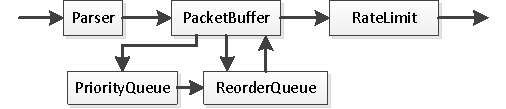
\includegraphics[width=1.0\columnwidth]{image/PFabric}
	\vspace{-0.30in}
	\caption{PFabric Element Graph}
	\vspace{-0.10in}
	\label{clicknp:fig:PFabric}
	%    
\end{figure}
}
